\documentclass[landscape]{article}
\usepackage{tikz}
\begin{document}
\begin{figure}[htb]
\centering\resizebox{\textwidth}{!}{%
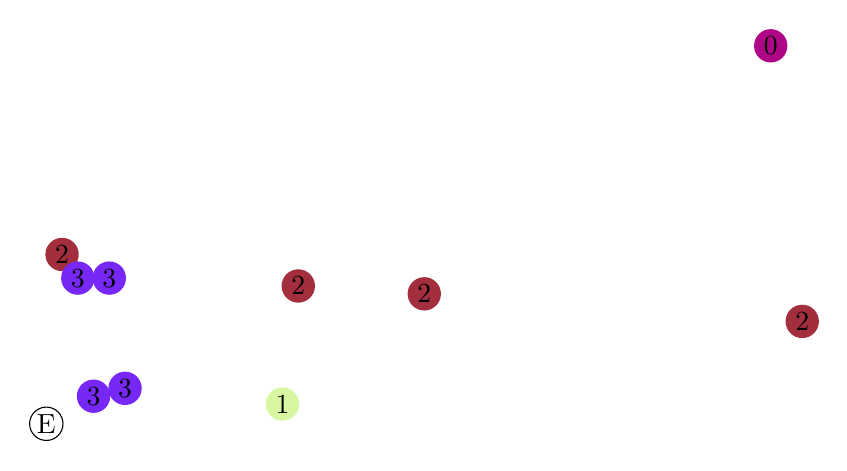
\begin{tikzpicture}
	\draw (0,0) circle (1.4ex);
	\node at (0,0) {E};
\definecolor{color0}{RGB}{175,6,135}
	\fill[color0] (9.200000000000001,4.800000000000001) circle (1.4ex);
	\node at  (9.200000000000001,4.800000000000001) {0};
\definecolor{color1}{RGB}{216,247,161}
	\fill[color1] (3.0,0.25) circle (1.4ex);
	\node at  (3.0,0.25) {1};
\definecolor{color2}{RGB}{162,46,62}
	\fill[color2] (0.2,2.15) circle (1.4ex);
	\node at  (0.2,2.15) {2};
	\fill[color2] (3.2,1.75) circle (1.4ex);
	\node at  (3.2,1.75) {2};
	\fill[color2] (4.800000000000001,1.6500000000000001) circle (1.4ex);
	\node at  (4.800000000000001,1.6500000000000001) {2};
	\fill[color2] (9.600000000000001,1.3) circle (1.4ex);
	\node at  (9.600000000000001,1.3) {2};
\definecolor{color3}{RGB}{120,40,246}
	\fill[color3] (0.6000000000000001,0.35000000000000003) circle (1.4ex);
	\node at  (0.6000000000000001,0.35000000000000003) {3};
	\fill[color3] (1.0,0.45) circle (1.4ex);
	\node at  (1.0,0.45) {3};
	\fill[color3] (0.8,1.85) circle (1.4ex);
	\node at  (0.8,1.85) {3};
	\fill[color3] (0.4,1.85) circle (1.4ex);
	\node at  (0.4,1.85) {3};
\end{tikzpicture}}
\end{figure}\end{document}